\section{实验评估与结果分析}
\subsection{评估流程设计}
为了验证抽取效果，项目构建了人工金标准数据，并采用 Precision、Recall 和 F1 作为标准评估指标。若 \(TP\)、\(FP\)、\(FN\) 分别表示真正例、假正例和漏检数，则
\[
P=\frac{TP}{TP+FP},\qquad R=\frac{TP}{TP+FN},\qquad F_1=\frac{2PR}{P+R}
\]
项目在评估脚本中先利用人工标注句子范围过滤预测结果，再进行集合碰撞，从而保证评估逻辑合理。

\begin{figure}[H]\centering
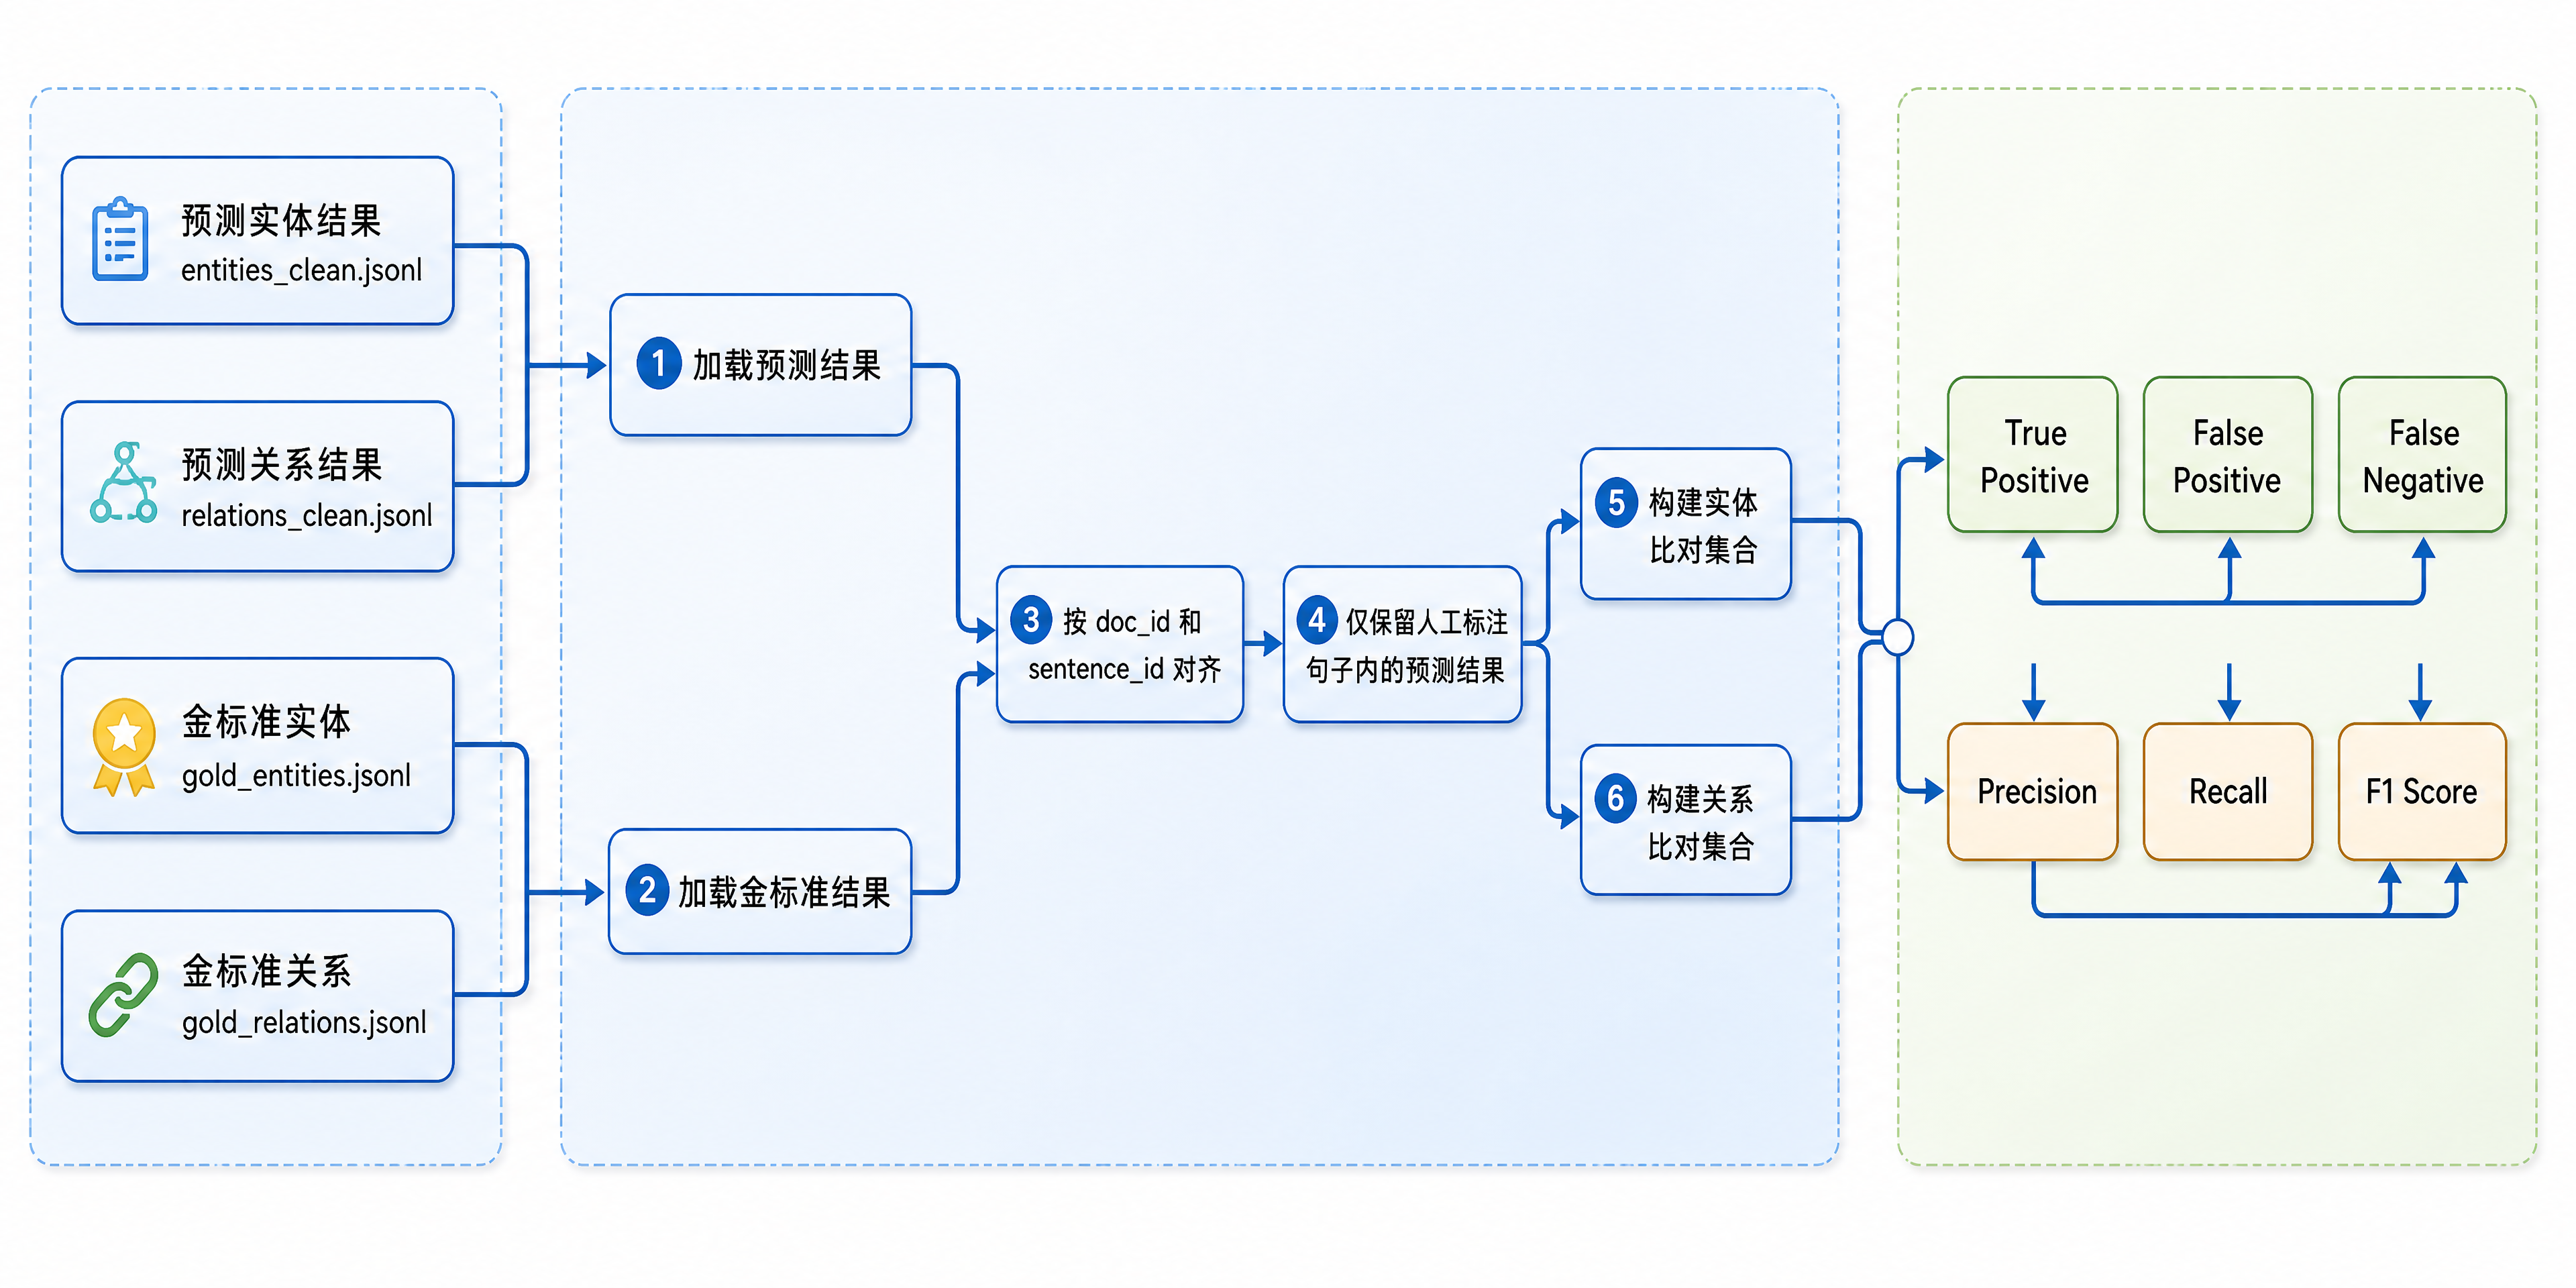
\includegraphics[width=0.88\textwidth]{figures/知识抽取算法评估流程图.png}
\caption{知识抽取算法评估流程图}
\end{figure}

\subsection{结果规模与统计分析}
从结果规模看，项目产生了 167846 条实体记录，并构建出约 1881 个知识节点和 11342 条知识关系。实体分布和关系分布统计表明，当前图谱在概念层次、结构组成和参数性能关联方面具有较好的覆盖度。整体结果说明，本项目已经具备了构建千级节点、万级关系图谱并进行前端可视化展示的能力。

在人工金标准评估中，实体抽取与关系抽取结果如表~\ref{tab:eval-all} 所示。可以看出，本项目在实体抽取任务上取得了较好的综合效果，Precision、Recall 和 F1 分别达到 87.12\%、97.52\% 和 92.03\%；关系抽取任务的 Precision、Recall 和 F1 分别达到 81.68\%、95.34\% 和 87.98\%。从指标分布看，系统整体呈现“召回率高于精确率”的特征，这说明当前方法具有较强的知识覆盖能力，同时仍存在一定的过抽取现象。

\begin{table}[H]
\centering
\caption{实体与关系抽取算法综合评估结果}
\label{tab:eval-all}
\renewcommand{\arraystretch}{1.28}
\resizebox{\textwidth}{!}{%
\begin{tabular}{>{\centering\arraybackslash}p{2.3cm}>{\centering\arraybackslash}p{2.1cm}>{\centering\arraybackslash}p{2.4cm}>{\centering\arraybackslash}p{2cm}>{\centering\arraybackslash}p{2cm}>{\centering\arraybackslash}p{1.8cm}}
\toprule
评估任务 & 真实数量 & 预测数量 & Precision & Recall & F1 \\
\midrule
实体抽取 & 444 & 497 & 87.12\% & 97.52\% & 92.03\% \\
关系抽取 & 1029 & 1201 & 81.68\% & 95.34\% & 87.98\% \\
\bottomrule
\end{tabular}%
}
\end{table}

图~\ref{fig:terminal} 展示了评估脚本在终端运行的实际输出结果，其各项实测指标（Precision、Recall、F1）与表~\ref{tab:eval-all} 中的统计数据完全对齐，进一步验证了系统评估逻辑的严谨性。

\begin{figure}[H]\centering
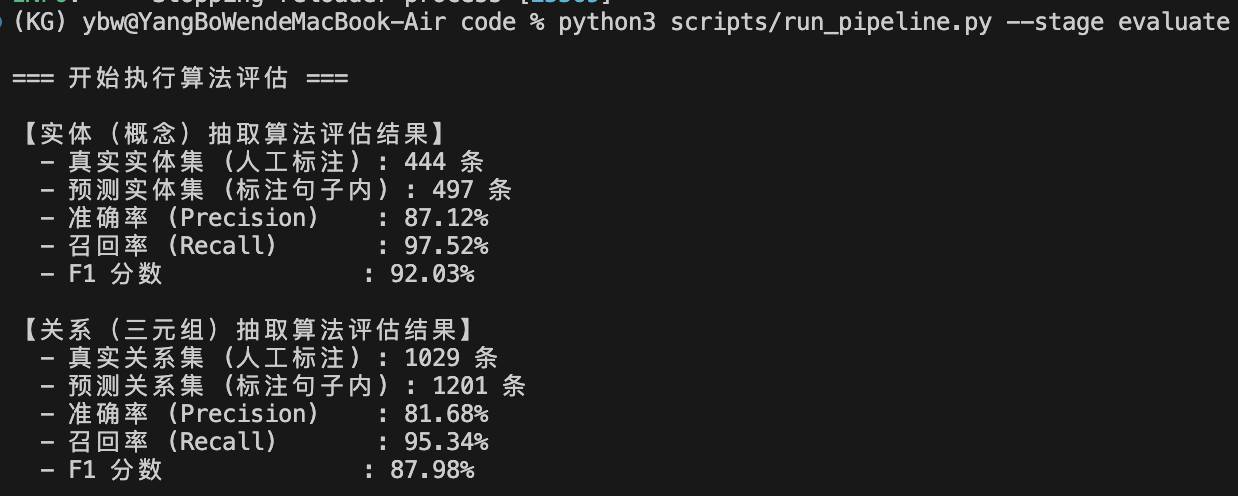
\includegraphics[width=0.82\textwidth]{figures/算法评估结果终端.png}
\caption{算法评估脚本终端运行输出结果}
\label{fig:terminal}
\end{figure}


从方法效果看，项目采用的混合方案在保持较高召回率的同时，通过术语清洗、实体二次过滤与关系多重约束提高了结果精度。说明“统计发现 + LLM 定稿 + 规则抽取”的路线在课程实验条件下具有较好的实用性和可解释性。

\subsection{算法评估结论}
综合两项任务的评估结果可以看出，实体抽取整体优于关系抽取。其主要表现为：实体抽取的 Precision、Recall 与 F1 均高于关系抽取，尤其是在 F1 指标上高出约 4 个百分点。造成这一差异的原因主要在于，实体抽取更多依赖术语词典、最长匹配和类型校验等相对稳定的规则，边界更明确、语义歧义相对较少；而关系抽取不仅依赖实体识别结果，还需要进一步判断两个实体之间是否真正存在稳定语义联系，因此更容易受到句式差异、触发词多义性和上下文复杂性的影响。

从系统定位看，这组实验结果说明本项目已经能够较稳定地支持变构飞行器领域知识的结构化组织任务。实体层面的高召回和高 F1 表明系统适合承担领域术语汇聚、概念归类和节点构建等基础工作；关系层面的较好表现则说明该系统已经具备构建初步语义连接网络的能力。虽然在复杂关系判定方面仍有进一步提升空间，但作为课程级领域知识组织原型，本系统已经能够较好地支撑知识图谱构建、可视化展示和后续扩展分析。

\subsection{误差来源与讨论}
从实体抽取结果看，召回率达到 97.52\%，说明术语词典与规则补充机制对领域概念具有较强覆盖能力，大部分人工标注实体能够被系统成功识别。Precision 为 87.12\%，略低于 Recall，说明当前词典匹配策略在保持高覆盖率的同时，也引入了少量假阳性实体。这类错误往往来自两个方面：一是部分通用术语在特定上下文中并非真正的领域实体，但仍被词典命中；二是个别短词项存在语义歧义，在句子中被错误识别为实体。

进一步分析可知，实体抽取误差与领域文献的表达复杂度密切相关。航空航天文献中存在大量带修饰语的复合术语、参数符号与自然语言混合表达、中文术语与英文缩写交替出现等现象，这些都容易造成实体边界不稳定。例如某些术语在一处以完整概念出现，而在另一处仅以简称出现，若别名映射覆盖不足，就可能产生重复识别或边界截断问题。此外，部分实体同时兼具概念属性和参数属性，其类型判断需要依赖上下文，而当前规则体系对这类细粒度歧义的区分能力仍有限。

从关系抽取结果看，Recall 达到 95.34\%，说明基于触发词的关系抽取机制能够较充分覆盖人工标注关系；但 Precision 为 81.68\%，低于实体抽取结果。这表明关系抽取比实体抽取更容易受到语义复杂性的影响。其主要原因在于：第一，同一句中两个实体虽然被触发词连接，但未必构成真正稳定的语义关系；第二，部分触发词如“基于”“采用”“影响”等在不同句式中语义范围较宽，容易引发过抽取；第三，当前方法主要面向句内显式关系，对隐式关系和复杂长距离关系的处理能力仍有限。

关系抽取的误差还反映出领域知识表达中“形式接近但语义不同”的典型问题。例如“某方法用于分析某参数变化”与“某参数影响某性能”在表层上都可能出现“用于”“影响”等触发词，但其真实语义角色并不相同。如果仅依赖浅层触发模式，很容易将方法关系、影响关系和适用关系相互混淆。此外，一些结构组成关系在句子中可能以列举方式出现，若缺少更强的依存约束或枚举边界识别，也可能将并列实体错误地连接为关系对。

从实验设计角度看，人工金标准本身也会对误差分析带来一定影响。目前标注集虽然已经能够反映系统总体效果，但在规模和覆盖面上仍有进一步扩展空间。尤其是在复杂长句、跨句承接、术语缩写和嵌套结构较多的样本上，如果标注数量进一步增加，将更有利于发现系统在边缘场景中的局限性。未来若能建立分层标注集，例如区分基础实体、复杂实体、显式关系和隐式关系，将有助于开展更细粒度的误差定位与模块优化。

总体而言，本项目在实体抽取和关系抽取两项任务上均取得了较好的实验结果，其中实体抽取 F1 达到 92.03\%，关系抽取 F1 达到 87.98\%，说明系统已经能够较稳定地支持变构飞行器领域知识图谱的构建任务。未来若进一步引入上下文建模、更细粒度的实体歧义消解策略以及轻量关系分类模型，预计仍有提升空间。
